\pdfoutput=1
\documentclass[11pt]{article}
\usepackage[a4paper,margin=2.4cm]{geometry}
\usepackage{amsmath,amssymb}
\usepackage{graphicx}
\usepackage[font=small,labelfont=bf]{caption}
\usepackage{subcaption}
\usepackage[colorlinks=true,allcolors=blue]{hyperref}
\usepackage{microtype}

\newcommand{\Iop}{\hat{I}}
\newcommand{\kB}{k_{\mathrm{B}}}

\title{\bfseries Classical records make the local arrow of time permanent}
\author{Mostfa Lejri\\[2pt]
\small Independent Researcher}
\date{\small Draft: \today}

\begin{document}
\maketitle

\begin{abstract}
\noindent
The microscopic laws of physics are invariant under time reversal, yet every observer records a fixed arrow of time. Decoherence theory explains how quantum systems acquire classical properties \cite{Zeh2007,Joos2003,Zurek2003}, and quantum Darwinism explains how those properties become objective through redundant environmental records \cite{Zurek2009,Riedel2012,Zurek2022}, but whether classicality, objectivity and the local orientation of time emerge together (and in what order) has remained an open question, studied so far in disconnected literatures \cite{Mlodinow2014,Chen2024,Guff2025,Aharonov2000}. Here we show, in an exactly solvable model in which the pointer observable is itself odd under time reversal (the circulation direction of a chiral ring monitored by a qubit bath), that the arrow of time is spontaneously broken: the unconditional entropy production vanishes identically, while the branch-relative entropy production equals exactly the information content of the environmental records. Both facts are instances of a model-independent theorem (Methods): for any microreversible dynamics with a two-valued time-reversal-odd branch variable, monitored so that the backward record statistics in a branch is the forward statistics of its antipode, the unconditional entropy production vanishes trajectory by trajectory and the branch-relative one equals the accumulated record distinguishability. The laws carry no arrow; conditioned histories do, and the ring is the minimal exactly solvable instance. Numerically, the orientation of the time-reversal-odd observable locks to the decoherence time across two decades of environment size, whereas Darwinian objectivity lags fourfold; branch polarization collapses onto a universal function of accumulated record distinguishability, with no hysteresis as coherent records degrade and revive. Only measurement converts this revocable arrow into a ratchet. Throughout, permanent means precisely this: immune to any subsequent recoherence of the original quantum records, once those records have been classicalized. Classicalization of records, not decoherence alone, is what makes the local arrow of time permanent.
\end{abstract}

\section*{Main}

Irreversibility is not written in the dynamical laws. Newtonian, quantum and relativistic dynamics are time-reversal symmetric, and the standard resolutions of this tension (the thermodynamic arrow from special initial conditions \cite{Albert2000}, the psychological arrow from the physics of memory \cite{Mlodinow2014}, the decoherent arrow from environmental monitoring \cite{Zurek2003,Guff2025}) share a common intuition: the arrow of time is carried by \emph{records}. Quantum Darwinism has made the record concept quantitative: a property of a system becomes objective when information about it proliferates redundantly into the environment, so that many observers can read it independently from small environmental fragments \cite{Zurek2009,Riedel2012,Zurek2022}. In parallel, stochastic thermodynamics has made irreversibility quantitative: the entropy production of a process equals the log-ratio of the probabilities of a trajectory and of its time reverse \cite{Maes2003,Callens2004,Landi2021}. These two quantifications (of objectivity and of irreversibility) have developed with essentially no contact. Recent proposals that classicality and the arrow of time co-emerge at a threshold, as an amplification-driven symmetry-breaking transition \cite{Aharonov2000}, have remained at the level of postulated order parameters. Here we connect the two frameworks in a model simple enough to be solved exactly, and specifically constructed so that the question is sharp: its pointer observable is odd under time reversal, so that fixing it \emph{is} breaking time-reversal symmetry locally.

\paragraph{An exactly solvable model with a T-odd pointer observable.}
The system is a single particle on a three-site ring, the minimal system with a well-defined sense of circulation. Its degenerate excited doublet consists of two states of opposite chirality, $|{+}\rangle$ and $|{-}\rangle$, carrying opposite currents; the current operator $\Iop$ commutes with the ring Hamiltonian and is odd under the antiunitary time-reversal operation, which exchanges the two chiralities. The environment is a bath of $N$ qubits coupled to the current, so that each qubit's precession records the circulation direction: the chiral states are exact pointer states, and the pointer observable is T-odd (Fig.~\ref{fig:model}). Prepared in the symmetric superposition $(|{+}\rangle+|{-}\rangle)/\sqrt2$, itself time-reversal invariant, the system decoheres without dissipation, and because the branch structure is exactly two-fold, every bipartite entropy has a closed form and the trajectory statistics of environmental measurements reduces to classical inference on a hidden fair coin: the branch. All numerical results below were validated against these closed forms at machine precision, and the redundancy curves reproduce the canonical partial-information plots of quantum Darwinism \cite{Riedel2012}. Throughout, objectivity is quantified by mutual-information redundancy in the original sense of quantum Darwinism \cite{Ollivier2004,Zurek2009}; in our exactly solvable two-branch model the strong refinements of objectivity (spectrum broadcast structure, strong quantum Darwinism \cite{Korbicz2021,Le2019}) essentially coincide with it, since the conditional environment states become orthogonal products, so the distinction carries no weight here. The model has a direct experimental cousin: superconducting flux qubits, whose clockwise/counterclockwise persistent-current superpositions realize precisely such a T-odd doublet \cite{Friedman2000}. The einselection of a degenerate chiral doublet has a venerable precedent: the environmental superselection of molecular handedness that resolves Hund's paradox \cite{Harris1981,Trost2009}. The crucial difference is the discrete symmetry involved: molecular handedness is parity-odd, so its fixation breaks P and carries no information about time; the circulation doublet is T-odd, and its fixation is precisely a local breaking of time-reversal symmetry, which is what permits the co-analysis with process irreversibility below.

\begin{figure}[t]
\centering
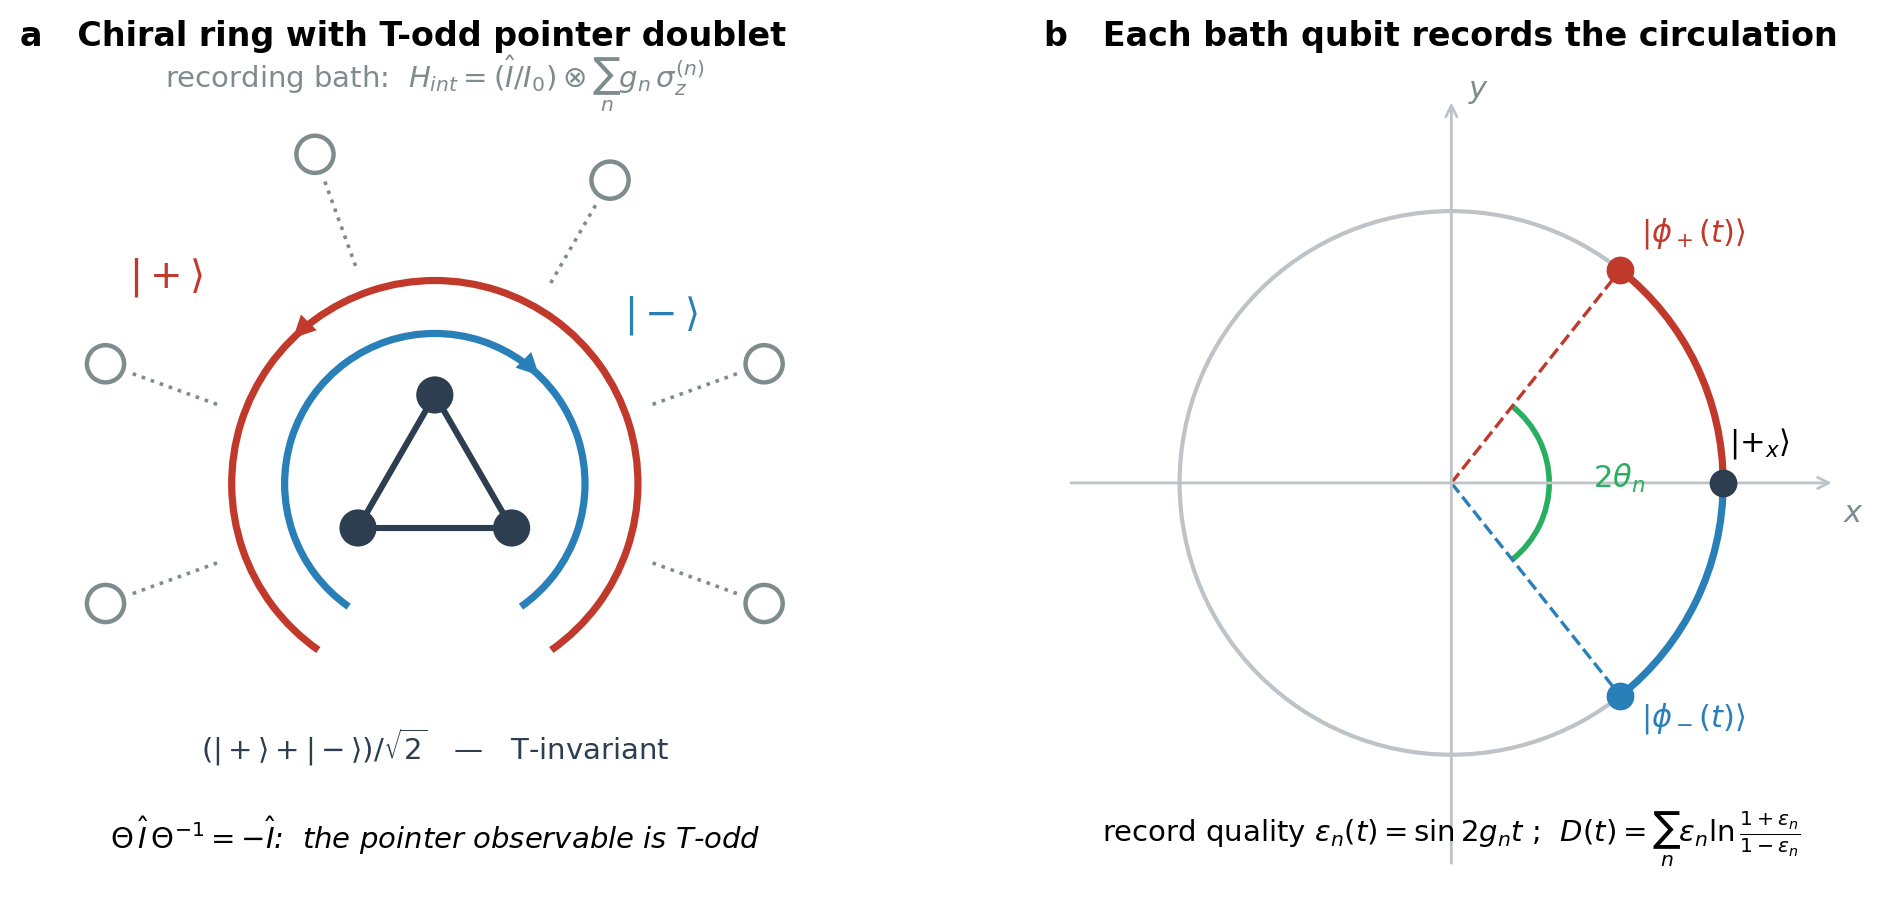
\includegraphics[width=0.95\linewidth]{fig1_schematic.png}
\caption{\textbf{A time-reversal-odd pointer observable.}
\textbf{a}, Three-site chiral ring with degenerate circulation doublet $|\pm\rangle$; a bath of qubits couples to the current, $H_{\mathrm{int}}=(\Iop/I_0)\otimes\sum_n g_n\sigma_z^{(n)}$; time reversal exchanges the branches, so the pointer observable is T-odd.
\textbf{b}, Conditional trajectories of one bath qubit on the Bloch equator: the growing angle between $|\phi_+(t)\rangle$ and $|\phi_-(t)\rangle$ constitutes the record, of quality $\varepsilon_n(t)=\sin 2g_nt$; the accumulated Kullback--Leibler distinguishability is $D(t)=\sum_n\varepsilon_n\ln[(1+\varepsilon_n)/(1-\varepsilon_n)]$.}
\label{fig:model}
\end{figure}

\paragraph{The arrow is spontaneously broken and equals record information.}
With the correct time-reversal operation (which flips both the current and the bath spins, leaving the total dynamics invariant) we prove two exact results (Methods). First, the unconditional stochastic entropy production vanishes identically, trajectory by trajectory: $\sigma[\xi]=0$ for every measurement record $\xi$. The ensemble has no arrow, exactly as a ferromagnet has no magnetization; the time asymmetry is spontaneously broken and exists only relative to a branch. We stress what distinguishes this from ordinary state-level T-breaking: a ferromagnet also einselects a T-odd observable, yet fixes no arrow. The claim here rests on the exact identity between the fixation of the state and the irreversibility of the process (the same variable $D$ governs both) and on the ratchet, which ties the permanence of the orientation to the modal status of the records; neither has a magnetic analogue. We use ``spontaneously broken'' in an operational, finite-size sense, exactly as finite-size einselection selects one of two symmetry-related pointer sectors: the ensemble remains rigorously T-symmetric while every conditioned history occupies one of two T-conjugate record sectors. We claim no thermodynamic phase transition; consistently, the transition does not sharpen with $N$ in the record variable. Second, for an observer within a branch (for whom the chirality is a fact that cannot be conjugated away) the branch-relative entropy production is strictly positive and equals, in expectation, the accumulated Kullback--Leibler distinguishability of the records,
\begin{equation}
\langle\sigma\rangle \;=\; D(t) \;=\; \sum_n D_{\mathrm{KL}}\!\big[p(r_n|s)\,\big\|\,p(r_n|{-}s)\big]:
\label{eq:identity}
\end{equation}
\textbf{the irreversibility of the process is identically the information content of the records about the direction of time-reversal-odd data}. We emphasize that the identity is not definitional: both sides have independent definitions from disjoint literatures, and the equality \emph{fails} for a T-even pointer observable, for which the branch-relative backward statistics coincides with the forward one and $\langle\sigma_s\rangle=0$ while $D$ grows. The equality encodes a physical fact specific to T-odd einselection: time reversal and branch exchange are the same operation. The associated integral fluctuation theorem $\langle e^{-\sigma}\rangle=1$ holds exactly and was confirmed numerically to one per cent for up to ten records, beyond which the estimator variance grows exponentially, as is generic \cite{Landi2021}. The identity \eqref{eq:identity} was confirmed by trajectory sampling to a relative deviation of $10^{-4}$, limited only by sampling.

\paragraph{The statement is model-independent.}
Nothing in the two results above uses the ring. They are instances of a general theorem (Methods): for \emph{any} microreversible dynamics carrying a two-valued branch variable that time reversal exchanges, monitored by records whose backward statistics in a branch equals the forward statistics of the antipodal branch, and prepared with a symmetric branch prior, the unconditional entropy production vanishes trajectory by trajectory and the branch-relative entropy production equals the Kullback--Leibler distinguishability of the full record, additively over records exactly when they are conditionally independent. The essential ingredients are therefore three: a T-odd two-valued pointer, branch-resolving records with the antipodal covariance, and a record-free initial condition. The three sites, the ring geometry, the coupling distribution and the bath size carry no weight; the chiral ring is the minimal exactly solvable instance, and the failure of the identity for a T-even pointer (for which conjugation fixes the branch instead of exchanging it, so $\langle\sigma_s\rangle = 0$ while $D$ grows) becomes a corollary rather than an observation. This is what licenses reading the mechanism as a principle: wherever a time-reversal-odd alternative is einselected by a recording environment, its fixation \emph{is} the local arrow, in the exact quantitative sense of Eq.~\eqref{eq:identity}.

\paragraph{Fixation precedes objectivity.}
Tracking three quantities through the transition (the decoherence of the system (entropy of the reduced state), the branch polarization $P$ (the mean magnitude of the conditional current, given the records), and the Darwinian redundancy $R_\delta$ (how many independent environmental fragments each supply the chirality)) reveals a strict temporal hierarchy (Fig.~\ref{fig:cotransition}). The polarization locks to the decoherence time: across bath sizes $N=8$ to $256$ the ratio of their half-rise times is $0.953\pm0.005$ pooled over ten disorder realizations per size, with a weak finite-size drift ($0.945\pm0.003$ at $N=8$) that saturates at $0.956\pm0.003$ beyond $N\approx64$. In the large-bath limit the two timescales are locked at a fixed sub-unit ratio, with polarization marginally leading, since the posterior over branches concentrates as soon as any record discriminates them, while the system's coherence requires the full product of overlaps to die. Redundancy, in contrast, lags fourfold: the chirality is \emph{fixed} long before it is \emph{objective}, consistent with the known continuation of redundancy growth after decoherence saturates \cite{Riedel2012}. The distribution of conditional currents evolves from unimodal, centred on zero (the time-symmetric phase) to sharply bimodal at the two chiralities (Fig.~\ref{fig:cotransition}b): the fingerprint of spontaneous T-symmetry breaking at the level of branches. All timescales scale as $N^{-1/2}$, and the transition does not sharpen relative to its own timescale: in the record variable there is no critical threshold, a point to which we return.

\begin{figure}[t]
\centering
\begin{subfigure}[t]{0.55\linewidth}

\includegraphics[width=\linewidth]{fig4_collision.png}
\caption{}
\end{subfigure}\hfill
\begin{subfigure}[t]{0.42\linewidth}
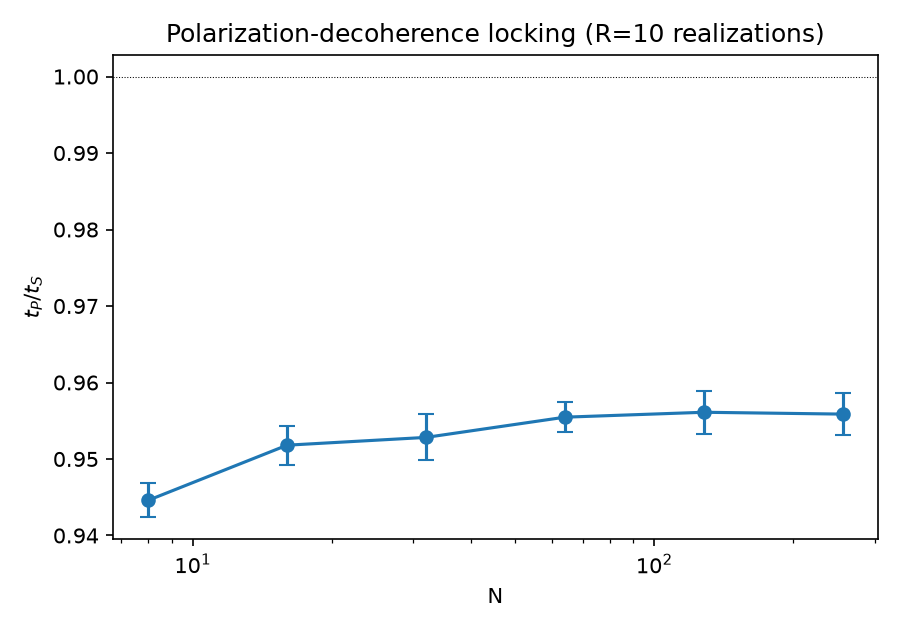
\includegraphics[width=\linewidth]{fig5b_ratio_errorbars.png}
\caption{}
\end{subfigure}\\[4pt]
\begin{subfigure}[t]{0.95\linewidth}
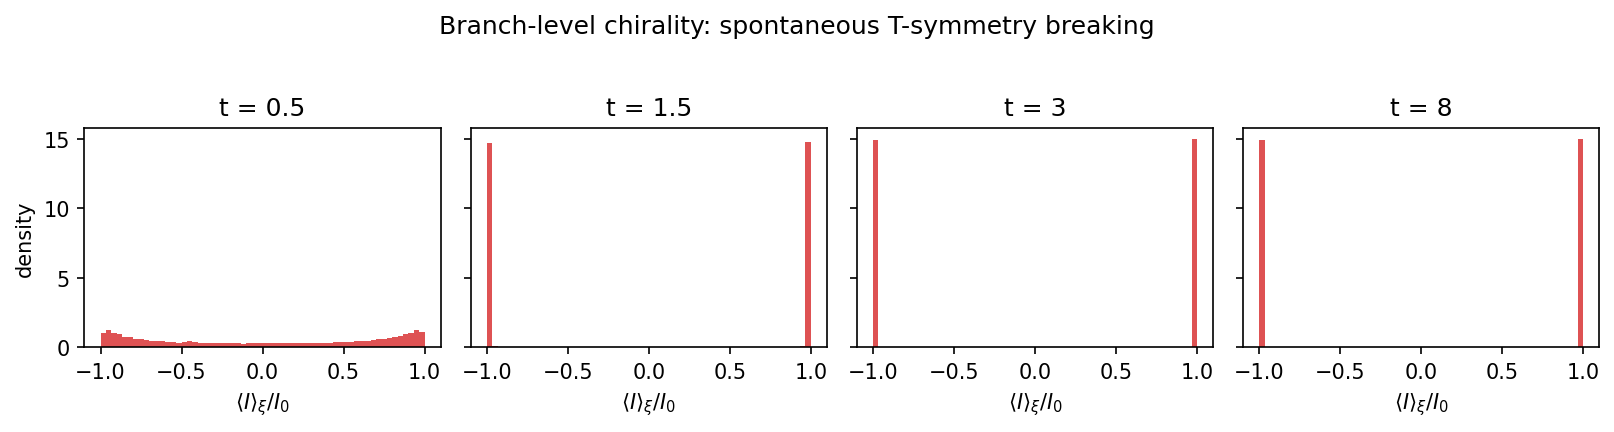
\includegraphics[width=\linewidth]{fig3_histograms.png}
\caption{}
\end{subfigure}
\caption{\textbf{Fixation precedes objectivity.}
\textbf{a}, Decoherence $S(\rho_S)$, branch polarization $P$, record distinguishability $D$ and redundancy $R_\delta$ versus time in the collision protocol ($N=120$): $P$ locks to $S$ while $R$ lags fourfold; the sampled entropy production $\langle\sigma\rangle$ (dots) falls exactly on $D$ [Eq.~\eqref{eq:identity}].
\textbf{b}, The ratio $t_P/t_S$ saturates at $0.956\pm0.003$ beyond $N\approx64$ (ten disorder realizations per size): locking at a fixed sub-unit ratio in the large-bath limit.
\textbf{c}, Distribution of the conditional current across branches: unimodal and time-symmetric before the transition, bimodal at $\pm I_0$ after; spontaneous T-symmetry breaking.}
\label{fig:cotransition}
\end{figure}

\paragraph{A universal curve, ridden in both directions.}
The deeper structure is that all these quantities are functionals of a single variable. Across bath sizes, coupling strengths and measurement protocols (including a collision protocol with entirely different dynamics) the branch polarization collapses onto one universal sigmoid $P(D)$ of the accumulated record distinguishability (Fig.~\ref{fig:collapse}a). This is explained by the exact identity above: entropy production, polarization and redundancy are all controlled by the same per-record divergences. In the snapshot protocol the polarization is by construction a functional of the instantaneous record qualities, so retracing is guaranteed; the non-trivial content of the degrading-record test (bath self-Hamiltonian, model still exactly solvable, $D(t)$ non-monotone) is that a \emph{single scalar} $D$ continues to suffice: the collapse is insensitive to the shape of the record-quality distribution even as records die and revive. The simplicity is the point: once the T-odd pointer reduces branch inference to a hidden binary variable, $D$ is the sufficient statistic for the posterior, and the universal curve is the operational translation of the local arrow rather than a numerical accident. The collapse is tight, with root-mean-square residual $0.005$ and maximum $0.024$ (bootstrap 95\% CI $[0.017, 0.024]$), and the hysteresis residual is at most $0.017$, decreasing monotonically with trajectory number, consistent with a sampling floor rather than any physical deviation (Fig.~\ref{fig:collapse}b). Coherent records make the local arrow fully revocable: when the environment recoheres, the branch orientation unfixes along exactly the path by which it fixed, with no detectable hysteresis.

\begin{figure}[t]
\centering
\begin{subfigure}[t]{0.49\linewidth}
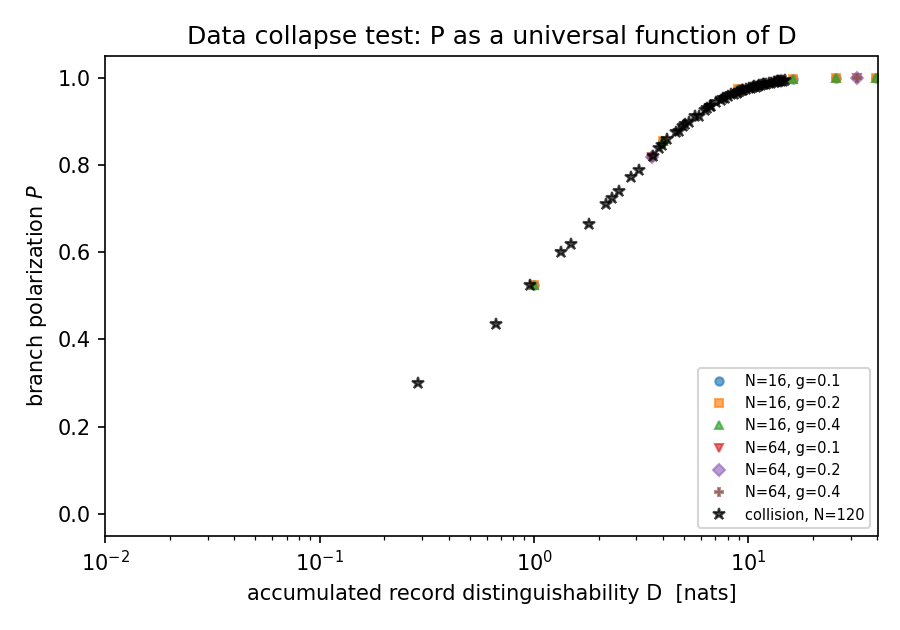
\includegraphics[width=\linewidth]{fig6_collapse.png}
\caption{}
\end{subfigure}\hfill
\begin{subfigure}[t]{0.49\linewidth}
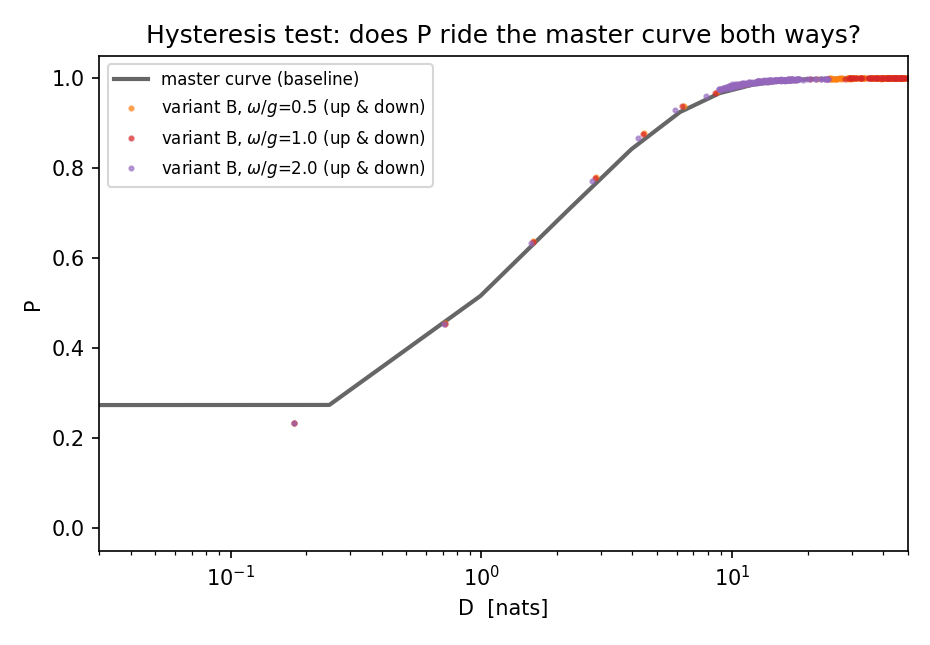
\includegraphics[width=\linewidth]{fig8_hysteresis.png}
\caption{}
\end{subfigure}
\caption{\textbf{One universal curve, no hysteresis.}
\textbf{a}, Branch polarization versus accumulated distinguishability for six parameter sets and two protocols: collapse onto a single sigmoid.
\textbf{b}, With degrading and reviving records (bath self-Hamiltonian, three ratios $\omega/\bar g$), the $(D,P)$ trajectory rides the same master curve up and down; maximal residual $0.017$, decreasing with trajectory number (sampling floor).}
\label{fig:collapse}
\end{figure}

\paragraph{The classicalization ratchet.}
The revocability disappears the moment records are classicalized. Running the identical degrading-record dynamics, but measuring each bath qubit once (converting its quantum record into a classical, permanent one) the polarization becomes monotone: each measured record is a click of a ratchet that no recoherence can undo (Fig.~\ref{fig:ratchet}). The contrast isolates the precise role of the quantum-to-classical transition in the arrow of time. Decoherence fixes the orientation of a T-odd observable within a branch; redundant proliferation makes that orientation objective; but only the classicalization of the records makes it \emph{permanent}. In the language of quantum Darwinism, the arrow of time inherits the modal status of the records that carry it.

\begin{figure}[t]
\centering
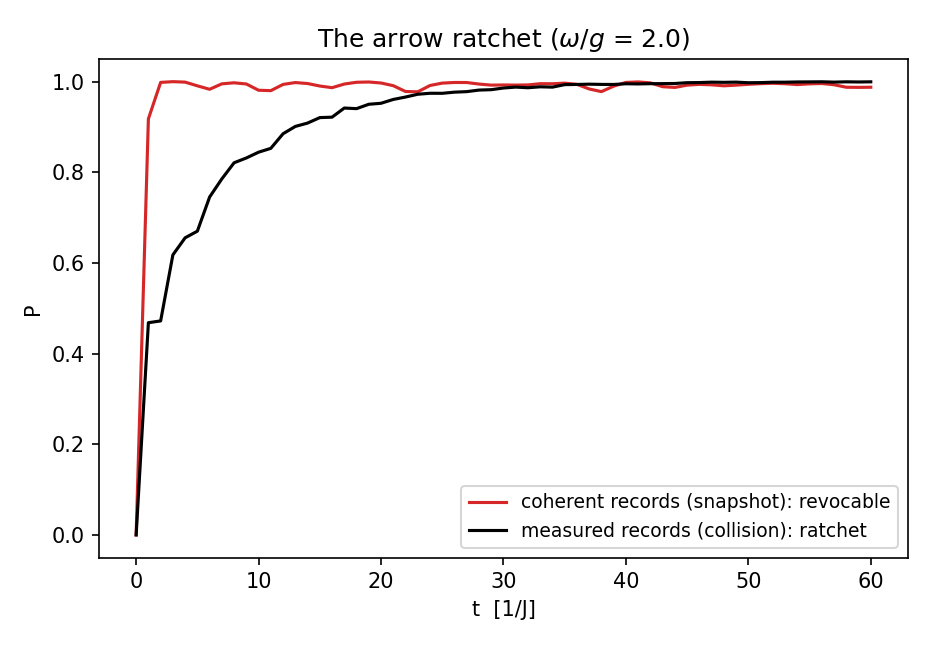
\includegraphics[width=0.62\linewidth]{fig9_ratchet.png}
\caption{\textbf{The classicalization ratchet.} Identical degrading-record dynamics, $\omega/\bar g=2$: with coherent records the polarization is revocable and oscillates; with each record measured once (classicalized), polarization is monotone; the arrow ratchets and cannot be undone by recoherence.}
\label{fig:ratchet}
\end{figure}

\begin{figure}[t]
\centering
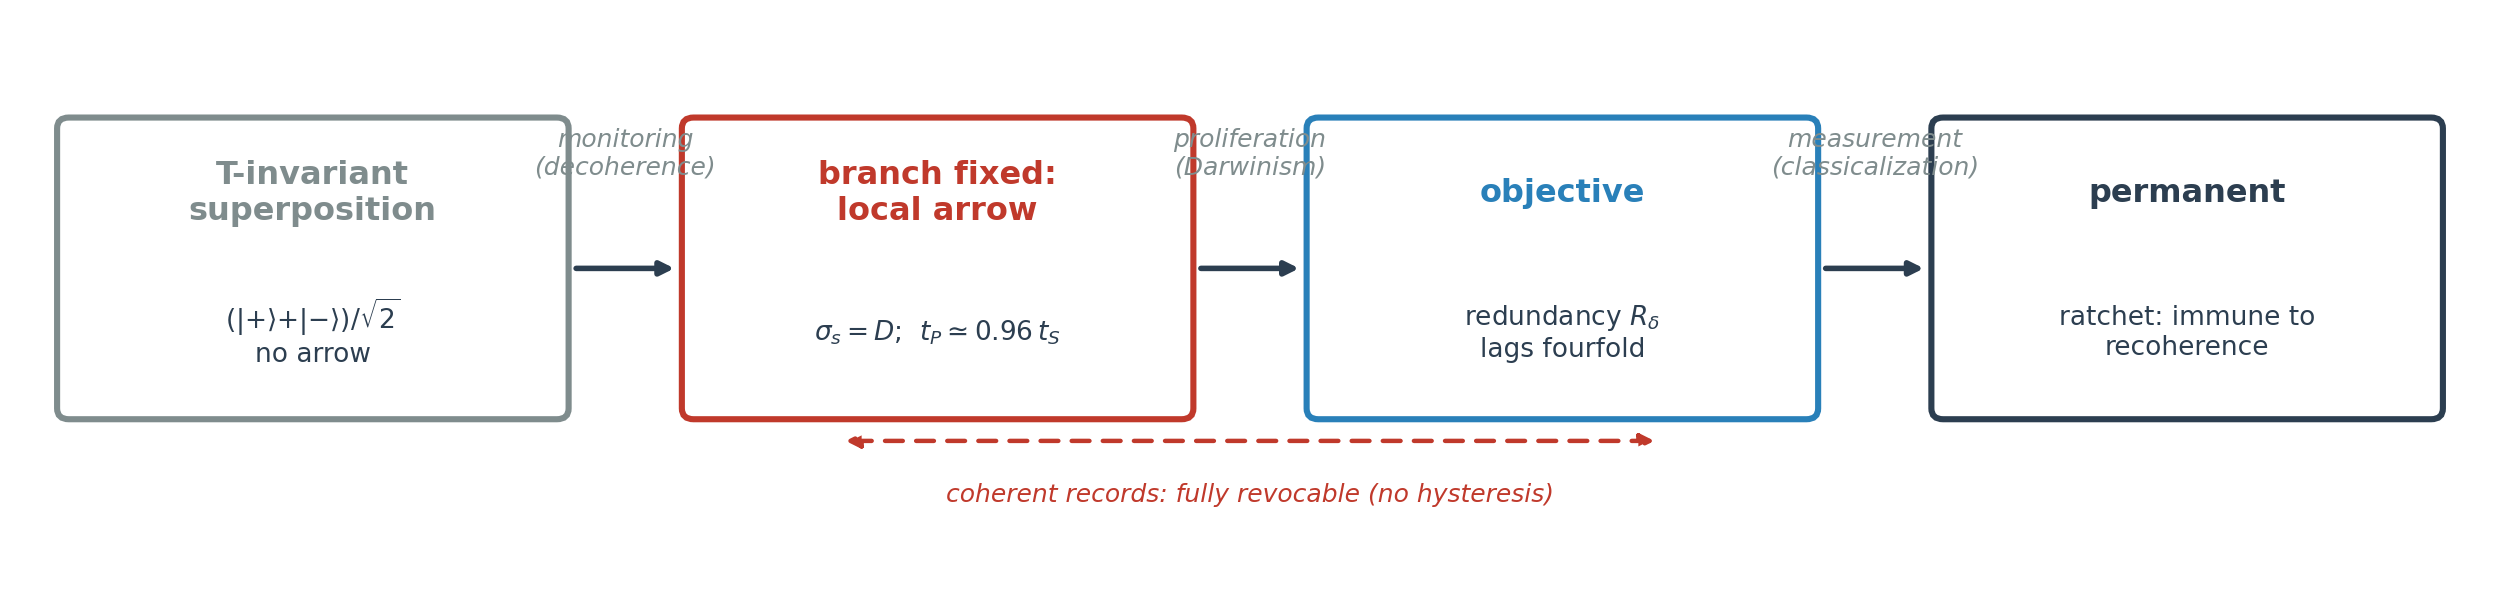
\includegraphics[width=0.98\linewidth]{fig2_sequence.png}
\caption{\textbf{The birth of a permanent local arrow.} Each stage is certified by a measured quantity of this paper: decoherence fixes the branch and the local arrow ($\sigma_s = D$, with $t_P \simeq 0.96\,t_S$); redundant proliferation makes it objective ($R_\delta$, lagging fourfold); while records stay coherent the arrow is fully revocable (no hysteresis on the master curve); only classicalization of the records makes it permanent (the ratchet).}
\label{fig:sequence}
\end{figure}

\paragraph{Discussion.}
Three limitations bound the claims. The ring is spatial, and its T-odd observable is a current: the model demonstrates decoherence-driven local breaking of time-reversal symmetry of the state, co-analysed with the irreversibility of the process. It does not model the emergence of time itself and, like all emergence-of-classicality arguments, presupposes a dynamics with a locality structure. Two clarifications sharpen this boundary. The mechanism itself is generic (any T-odd observable monitored by a recording environment undergoes the same branch-level fixation, and records beget records), so a contagion of local arrows into a consistent global one is a natural conjecture; but what would propagate is the thermodynamic orientation, the direction of record accumulation, not the randomly einselected chirality, and demonstrating alignment across many systems requires a multi-system model we have not built. And the asymmetry that does propagate is inherited from the initial condition: the record-free product state of the bath is a Past Hypothesis in miniature \cite{Chen2024}, so the model derives the local arrow \emph{given} an initially record-free environment, and defers the origin of that condition to cosmology, where it belongs \cite{Halliwell1994}. The branch-relative construction sits naturally in decoherent-histories quantum mechanics \cite{GellMann1993}: the two branches form an exactly decohering set of coarse-grained histories, and $\sigma_s$ is a property of an individual history rather than of the ensemble. The possibility that emergent arrows point in different directions in different regions or epochs, raised at the level of quantum cosmology \cite{Hartle2013}, here acquires a microscopic, record-level carrier. Complementary channel-level notions of irreversible classicality, such as the monotone contraction of coherence functionals relative to a fixed conjugation \cite{Gil2026}, address the approach to classicality of the map rather than the T-symmetry of the state, and are compatible with the present state-level analysis. A related objection deserves a direct answer: the model contains no heat, work, or dissipation, so one may ask whether $\sigma$ deserves the name entropy production at all. That is by design: the construction isolates the informational component of the arrow with zero energetic confound, within the measurement-inclusive framework of stochastic thermodynamics \cite{Landi2021}; adding dissipative channels would add entropy production, not replace the record term. The branch-relative definition of entropy production is a choice. We defend it on the grounds that the alternative of conjugating the branch is unavailable to any observer whose memories are themselves records within the branch \cite{Mlodinow2014}, and yields identically zero information. Finally, our universal sigmoid is smooth: standard decoherence plus redundancy produces no sharp threshold in the record variable. This sharpens, rather than undermines, the testability of proposals in which the quantum--classical transition is a genuine critical phenomenon \cite{Aharonov2000}: any observed threshold-like disappearance of interference at a critical noise or amplification level would be a departure from the exactly solvable baseline established here. The flux-qubit realization of the chiral doublet \cite{Friedman2000} suggests that measuring the polarization--distinguishability curve, and the ratchet contrast, is within reach of existing circuit-QED techniques. More broadly, the model turns a metaphysical question (when does time acquire a direction?) into an operational one: the local arrow is fixed when, and only for as long as, the environment can tell a process from its time reverse; it becomes objective when many can tell independently; and it becomes irrevocable only when their records do.

\section*{Methods}

\paragraph{Model.}
$H = H_S\otimes\mathbb1 + (\Iop/I_0)\otimes\sum_n g_n\sigma_z^{(n)}$ ($+\sum_n\omega_n\sigma_x^{(n)}$ for degrading records), with $H_S$ the three-site hopping Hamiltonian, $\Iop$ the current operator, $[H_S,\Iop]=0$, $I_0=\sqrt3 J$. Couplings $g_n$ drawn uniformly from $[\bar g/2, 3\bar g/2]$. Bath initialized in $|{+_x}\rangle^{\otimes N}$. The conserved chirality reduces the global state to two branches, each a product over bath qubits; all bipartite reduced states have rank $\le2$, giving closed-form entropies (binary entropy of $(1\pm|c|)/2$ with $c$ the appropriate product of single-qubit overlaps). Brute-force state-vector evolution at $N=8$ agrees with the closed forms to $5\times10^{-14}$. Two remarks on the status of these idealizations. Exact degeneracy of the doublet is not fine-tuning but the statement of the problem: a splitting between $|+\rangle$ and $|-\rangle$ is a current bias, itself T-odd, so imposing it would break time-reversal symmetry in the law rather than let it break spontaneously, exactly as a ferromagnet is studied at zero external field. And the legitimate T-even perturbation, a tunneling $\Delta$ between the chiralities, places the model in the standard competition between pointer states and energy eigenstates: in the strong-monitoring regime $g\gg\Delta$ (the quantum measurement limit underlying pure-dephasing models since their inception \cite{Zurek2003}) chirality einselection survives approximately; quantifying that crossover is left for future work. Mathematically, tracing out the ring reduces the construction to the exactly solvable central-spin dephasing model that has anchored einselection studies since their origin \cite{Zurek1981,Riedel2012}; the new ingredient is not the mathematics but the symmetry: the central ``spin'' is a chiral doublet whose basis states are exchanged by time reversal, and the monitored observable is T-odd, which is what opens the co-analysis with process irreversibility.

\paragraph{Time reversal.}
Baseline: $\Theta = K_{\mathrm{ring}}\otimes(i\sigma_yK)^{\otimes N}$, under which $\Iop\to-\Iop$, $\sigma_z\to-\sigma_z$, hence $\Theta H\Theta^{-1}=H$. With the bath self-Hamiltonian, $\Theta = K_{\mathrm{ring}}\otimes(\sigma_xK)^{\otimes N}$. Backward protocol: $\Theta$-imaged preparation, motion-reversed evolution, $\Theta$-imaged detectors retaining forward labels; the T-oddness of the record datum enters through the trajectory conjugation $\tilde\xi$ (reversed order, $\tilde r_n=-r_n$).

\paragraph{Entropy production.}
Collision protocol: qubit $n$ interacts during $[t_{n-1},t_n]$, measured in the $\sigma_y$ (Helstrom-optimal) basis. $P(r_n|s)=(1+r_ns\varepsilon_n)/2$ with $\varepsilon_n=\sin(2g_n\Delta t)$ (baseline) or $\sqrt{1-|c_n|^2}$ (degrading records). $\sigma[\xi]=\ln P_{\mathrm{fwd}}(\xi)-\ln P_{\mathrm{bwd}}(\tilde\xi)$ vanishes identically after branch averaging (double sign flip plus symmetric prior). Branch-relative: $\sigma_s[\xi]=\sum_n\ln[(1+r_ns\varepsilon_n)/(1-r_ns\varepsilon_n)]$, with $\langle\sigma_s\rangle=\sum_n\varepsilon_n\ln[(1+\varepsilon_n)/(1-\varepsilon_n)]=D$. All six formal steps were verified by an independent numerical suite (machine precision; repository).

\paragraph{Branch Arrow Theorem.}
Hypotheses: (H1) microreversible dynamics with a two-valued branch variable $s = \pm 1$ exchanged by the antiunitary $\Theta$; (H2) record trajectories $\xi$ with conjugate $\tilde\xi$ (reversed order, T-odd data) satisfying the antipodal covariance $P_{\mathrm{fwd}}(\xi|{-s}) = P_{\mathrm{fwd}}(\tilde\xi|s)$, and a $\Theta$-imaged backward protocol, so that $P_{\mathrm{bwd}}(\tilde\xi|s) = P_{\mathrm{fwd}}(\xi|{-s})$; (H3) symmetric branch prior. Conclusions: (a) $\sigma[\xi] = \ln P_{\mathrm{fwd}}(\xi) - \ln P_{\mathrm{bwd}}(\tilde\xi) = 0$ for every $\xi$; (b) $\sigma_s[\xi] = \ln[P(\xi|s)/P(\xi|{-s})]$, hence $\langle\sigma_s\rangle = D_{\mathrm{KL}}[P(\cdot|s)\,\|\,P(\cdot|{-s})] \ge 0$, reducing to the additive form of Eq.~\eqref{eq:identity} exactly when the records are conditionally independent. Proof of (a): $P_{\mathrm{bwd}}(\tilde\xi) = \tfrac12\sum_s P_{\mathrm{fwd}}(\xi|{-s}) = P_{\mathrm{fwd}}(\xi)$. Proof of (b): $P_{\mathrm{bwd}}(\tilde\xi|s) = P(\xi|{-s})$ by (H2), and the expectation of the log-likelihood ratio under $P(\cdot|s)$ is the stated divergence. Conditional independence is nowhere required; it is used only to write the divergence as a sum. The theorem was verified as an independent gate on randomly drawn \emph{correlated} record laws satisfying (H2) (conclusions (a) and (b) at machine precision; additivity gap up to $1.2$ nats for correlated laws, zero for product laws) and on a T-even control (conjugation fixing the branch: $\sigma_s \equiv 0$ while the marginal distinguishability grows), scripts in the repository. The chiral ring satisfies (H1)--(H3) by the constructions above.

\paragraph{Statistics.}
Reported errors are standard deviations over ten independent disorder realizations of the couplings. Trajectory sampling: $5\times10^4$ per curve point (up to $3\times10^5$ for the hysteresis floor test), making Monte-Carlo noise subdominant. Master curve for collapse residuals: quantile-binned running median over 200 time points per realization; confidence interval on the maximal residual by bootstrap (200 resamples).

\paragraph{Observables.}
Redundancy $R_\delta$: smallest fragment fraction whose average mutual information with the system reaches $(1-\delta)S(\rho_S)$, $\delta=0.1$, 150 fragment samples per size. Polarization: posterior $q(\xi)$ over branches from Bayes on the sampled records; the conditional current obeys $\langle\Iop\rangle_\xi=I_0(2q-1)$ exactly (verified against exhaustive enumeration at $N=4$); $P=\mathbb E|2q-1|$, $3{,}000$--$20{,}000$ trajectories. Timescales: interpolated 50\% crossings; widths: 10--90\% rise.

\paragraph{Data and code availability.}
All code ($\approx$700 lines, Python/NumPy) and generation scripts for every figure are available at \url{https://github.com/lejrimostfa/chiral-ring}; every figure regenerates from fixed seeds by a single command.


\section*{Acknowledgments}
This work made extensive use of Anthropic's Claude (a large language model) as a research assistant, for model design discussions, derivations, code, and manuscript drafting. Every analytic claim was verified by an independently recoded numerical suite to machine precision. This verification loop caught and corrected one convention error during development. The author reviewed all derivations and takes sole and full responsibility for the content.

\begin{thebibliography}{99}\small
\bibitem{Zeh2007} H.~D. Zeh, \emph{The Physical Basis of the Direction of Time} (Springer, 2007).
\bibitem{Joos2003} E.~Joos \emph{et al.}, \emph{Decoherence and the Appearance of a Classical World in Quantum Theory} (Springer, 2003).
\bibitem{Zurek1981} W.~H. Zurek, Pointer basis of quantum apparatus: Into what mixture does the wave packet collapse?, \emph{Phys. Rev. D} \textbf{24}, 1516 (1981); Environment-induced superselection rules, \emph{Phys. Rev. D} \textbf{26}, 1862 (1982).
\bibitem{Zurek2003} W.~H. Zurek, Decoherence, einselection, and the quantum origins of the classical, \emph{Rev. Mod. Phys.} \textbf{75}, 715 (2003).
\bibitem{Ollivier2004} H.~Ollivier, D.~Poulin, W.~H. Zurek, Objective properties from subjective quantum states, \emph{Phys. Rev. Lett.} \textbf{93}, 220401 (2004).
\bibitem{Zurek2009} W.~H. Zurek, Quantum Darwinism, \emph{Nat. Phys.} \textbf{5}, 181 (2009).
\bibitem{Riedel2012} C.~J. Riedel, W.~H. Zurek, M.~Zwolak, The rise and fall of redundancy in decoherence and quantum Darwinism, \emph{New J. Phys.} \textbf{14}, 083010 (2012).
\bibitem{Zurek2022} W.~H. Zurek, Quantum theory of the classical, \emph{Entropy} \textbf{24}, 1520 (2022).
\bibitem{Mlodinow2014} L.~Mlodinow, T.~A. Brun, Relation between the psychological and thermodynamic arrows of time, \emph{Phys. Rev. E} \textbf{89}, 052102 (2014).
\bibitem{Chen2024} J.~Al-Khalili, E.~K. Chen, The decoherent arrow of time and the entanglement past hypothesis, \emph{Found. Phys.} \textbf{54}, 49 (2024).
\bibitem{Guff2025} T.~Guff, C.~U. Shastry, A.~Rocco, Emergence of opposing arrows of time in open quantum systems, \emph{Sci. Rep.} \textbf{15}, 3658 (2025).
\bibitem{Aharonov2000} D.~Aharonov, Quantum to classical phase transition in noisy quantum computers, \emph{Phys. Rev. A} \textbf{62}, 062311 (2000).
\bibitem{Albert2000} D.~Z. Albert, \emph{Time and Chance} (Harvard Univ. Press, 2000).
\bibitem{Maes2003} C.~Maes, K.~Neto\v{c}n\'y, Time-reversal and entropy, \emph{J. Stat. Phys.} \textbf{110}, 269 (2003).
\bibitem{Callens2004} I.~Callens, W.~De Roeck, T.~Jacobs, C.~Maes, K.~Neto\v{c}n\'y, Quantum entropy production as a measure of irreversibility, \emph{Physica D} \textbf{187}, 383 (2004).
\bibitem{Landi2021} G.~T. Landi, M.~Paternostro, Irreversible entropy production: from classical to quantum, \emph{Rev. Mod. Phys.} \textbf{93}, 035008 (2021).
\bibitem{Gil2026} J.~J. Gil, Intrinsic pointer basis and irreversible classicality from coherence contraction, arXiv:2604.23304 (2026).
\bibitem{Harris1981} R.~A. Harris, L.~Stodolsky, On the time dependence of optical activity, \emph{J. Chem. Phys.} \textbf{74}, 2145 (1981).
\bibitem{Trost2009} J.~Trost, K.~Hornberger, Hund's paradox and the collisional stabilization of chiral molecules, \emph{Phys. Rev. Lett.} \textbf{103}, 023202 (2009).
\bibitem{GellMann1993} M.~Gell-Mann, J.~B. Hartle, Classical equations for quantum systems, \emph{Phys. Rev. D} \textbf{47}, 3345 (1993).
\bibitem{Hartle2013} J.~B. Hartle, The quantum mechanical arrows of time, arXiv:1301.2844 (2013).
\bibitem{Halliwell1994} J.~J. Halliwell, J.~P\'erez-Mercader, W.~H. Zurek (eds.), \emph{Physical Origins of Time Asymmetry} (Cambridge Univ. Press, 1994).
\bibitem{Korbicz2021} J.~K. Korbicz, Roads to objectivity: quantum Darwinism, spectrum broadcast structures, and strong quantum Darwinism, \emph{Quantum} \textbf{5}, 571 (2021).
\bibitem{Le2019} T.~P. Le, A.~Olaya-Castro, Strong quantum Darwinism and strong independence are equivalent to spectrum broadcast structure, \emph{Phys. Rev. Lett.} \textbf{122}, 010403 (2019).
\bibitem{Friedman2000} J.~R. Friedman \emph{et al.}, Quantum superposition of distinct macroscopic states, \emph{Nature} \textbf{406}, 43 (2000).
\end{thebibliography}

\end{document}
